\section{Evaluation Methodology}
\label{sec:evaluation-methodology}
\fxfatal{More formal approach, see \cite{Sitter:2004}}

In the previous chapter the field of information extraction was presented. The process of IE does not only require the extraction itself, but also needs to evaluate the relevance of localized facts for the respective domain. Thus, a quality assessment is required, which focuses on the advancement of development and the juxtaposition of approaches. The evaluation is the formulation of new problems which have to be integrated into the development \cite{Linsmayr:2010}. The methodology of the evaluation is described in this chapter.

Evaluation has always been an important part in designing, implementing, testing and developing \gls{IE} systems. It's crucial to have reliable indicators to ensure a continuous improvement in system performances. This chapter aims to provide an overview of the most important and well discussed performance metrics which will be implemented in the framework. For information about the implementation details of the scoring metrics please consult chapter \ref{sec:design} (pp. \pageref{sec:design}ff.).

\subsection{Performance measures}
A typical way to evaluate an IE system is by using a confusion matrix. This is a well-known
technique of counting results. Figure \ref{tab:confusion-matrix} shows a confusion matrix \cite{Sitter:2004}.

\begin{table}[H]
\centering
\begin{tabular}{c|ccc}
	& \multicolumn{2}{c}{\shortstack{\textbf{Actual class} \\ (Observation)}} \\
	\toprule
	\multirow{6}{*}{\shortstack{\textbf{Predicted class} \\ (Expectation)}} & \textbf{\textit{tp}}  & \cellcolor{gray!15} \textbf{\textit{fp}} \\
	& (true positive) & \cellcolor{gray!15} (false positive) \\
	& Correct result & \cellcolor{gray!15} Unexpected result \\
	& \cellcolor{gray!15} \textbf{\textit{fn}} & \textbf{\textit{tn}} \\
	& \cellcolor{gray!15} (false negative) & (true negative) \\
         & \cellcolor{gray!15} Missing result & Correct absence of result
\end{tabular}
\caption{Confusion matrix}
\label{tab:confusion-matrix}
\end{table}

For each extracted entity, we have to evaluate if it is correct (and thus a true positive) or not (and thus a false positive). The false negative in the matrix is the number of entities that should have been extracted, but haven't. In IE applications, the true negative is usually not used \cite{Sitter:2004} because we typically do not know what a \enquote{true negative} is. Unlike in document classification, a \enquote{bad tuple} does not exist apriori in a document. It only exists because the extraction system can extract it \cite{Ipeirotis:2007}.

Another way to calculate performance measures is based on the notation proposed by \citeauthor{Makhoul:1999} \cite{Makhoul:1999}:

\begin{table}[H]
\centering
\begin{tabular*}{\textwidth}{ll}
	\toprule
	\textbf{Symbol} & \textbf{Meaning} \\
	\midrule
	N & total number of slots in the reference \\
	M & total number of slots in the hypothesis \\
	C & number of correct slots \\
	S & number of substitutions (incorrect slots) \\
	D & number of deletions (missing slots or false rejections) \\
	I & number of insertions (spurious slots or false acceptances) \\
	\bottomrule
\end{tabular*}
\end{table}

\gls{IE} has been, according to \cite{Chinchor:1998}, traditionally defined as the extraction of information from a text in the form of text strings and processed text strings which are placed into slots labeled to indicate the kind of information that can fill them. To summarize: Slots, in this context, can be understood as the extraction target for entities.

The most used evaluation measures in \gls{IE} are recall, precision and F-measure. Some additional ones, like Error per response fill and  Slot error rate, were proposed by \cite{Chinchor:1995} and \cite{Makhoul:1999}.

\subsubsection{Precision}
The \textit{precision} (\ensuremath{\pi} or P), also called Sensitivity, is defined as the percentage of correctly retrieved data in the hypothesis \cite{Carstensen:2010}. 

\begin{figure}[H]
\begin{displaymath}
	\pi = \frac{\textit{tp}}{\textit{tp} + \textit{fp}} = \frac{C}{C+S+I}
\end{displaymath}
\caption{Precision formula}
\end{figure}

For example, a precision of .9 can be translated to: 90\% of the slots in the hypothesis were extracted correctly.

\subsubsection{Recall}
The \textit{recall} (\ensuremath{\rho} or R), also referred to as the \gls{PPV}, describes the completeness of an extraction, which is determined by the ratio of correctly predicted results to all correct results \cite{Carstensen:2010}.

\begin{figure}[H]
\begin{displaymath}
	\rho = \frac{\textit{tp}}{\textit{tp} + \textit{fn}} = \frac{C}{C+S+D}
\end{displaymath}
\caption{Recall formula}
\end{figure}

An exemplary recall of .9 can be interpreted as follows: 90\% of the slots in the reference were extracted correctly.

Figure \ref{fig:recall-precision} shows a graphical interpretation of precision and recall. The relevant items are to the left of the straight line while the retrieved items are within the oval. The red regions represent errors. On the left these are the relevant items not retrieved (false negatives), while on the right they are the retrieved items that are not relevant (false positives). Precision and recall are the quotient of the left green region by respectively the oval (horizontal arrow) and the left region (diagonal arrow) \cite{Wikipedia:Precision_and_recall}.

\begin{figure}[H]
\centering
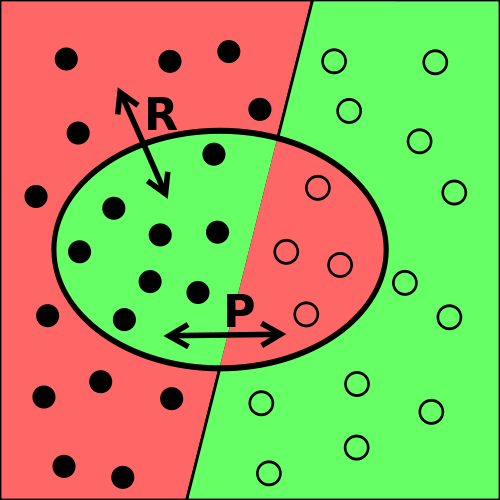
\includegraphics[width=0.35\textwidth]{recall-precision.png}
\caption{Recall and precision example figure \cite{Wikipedia:Precision_and_recall}}
\label{fig:recall-precision}
\end{figure}

\subsubsection{F-measure}
The \textit{F-measure} (F), or  balanced F-score or $\textit{F}_\textit{1}$ score, was introduced to combine \textit{precision} and \textit{recall} into a single measure.

\begin{figure}[H]
\begin{displaymath}
	F_1 = 2 \cdot \frac{\pi \cdot \rho}{\pi + \rho} = \frac{2 \cdot C}{N + M}
\end{displaymath}
\caption{F-measure formula}
\end{figure}

Figure \ref{fig:fbeta-score} shows the more general formula of $\textit{F}_\beta$-score, which contains a parameter $\beta$ to control the balance between \textit{precision} and \textit{recall}. When $\beta$ = 1, $\textit{F}_\textit{1}$ comes to be equivalent to the harmonic mean of $\pi$ and $\rho$. If $\beta$ > 1, F becomes more recall-oriented and if $\beta$ < 1, it becomes more precisionoriented \cite{Sasaki:2007}.

\begin{figure}[H]
\begin{displaymath}
	F_\beta = (1+\beta^2) \cdot \frac{\pi \cdot \rho}{(\beta^2 \cdot \pi) + \rho}, (0 \le \beta \le +\infty)
\end{displaymath}
\caption{$\textit{F}_\beta$-score formula \cite{Chinchor:1992}}
\label{fig:fbeta-score}
\end{figure}

$\textit{F}_\beta$ measures the effectiveness of retrieval with respect to a user who attaches $\beta$ times as much importance to recall as precision \cite{Rijsbergen:1979}.

Another commonly used formula for the F-measure is shown in \ref{fig:falpha-score}. In contrast to Rijsbergen's formula, the balance parameter $\alpha$ is balanced when it's set to 0.5.

\begin{figure}[H]
\begin{displaymath}
	F_\alpha = \frac{\pi \cdot \rho}{(1-\alpha) \cdot \pi + \alpha \cdot \rho}, (0 \le \alpha \le 1)
\end{displaymath}
\caption{$\textit{F}_\alpha$-score formula \cite{Makhoul:1999}}
\label{fig:falpha-score}
\end{figure}

\subsubsection{Error measure}
Since \textit{F} is a figure of merit, the higher its value the better we consider the performance of the system. We can then define \textit{E} = 1 – $F_\alpha$ as a corresponding \textit{error measure} \cite{Makhoul:1999}:

\begin{figure}[H]
\begin{displaymath}
	E = 1 - F_\alpha = \frac{S + (1-\alpha) \cdot D + \alpha \cdot I}{(1-\alpha) \cdot N + \alpha \cdot M}, (0 \le \alpha \le 1)
\end{displaymath}
\caption{Error measure formula}
\label{eq:error-measure}
\end{figure}

\subsubsection{Error per Response Fill}
The \textit{Error per Response Fill} (\textit{ERR}) is based on the Error measure and removes the deweighting of \textit{D} and \textit{I} by simply removing the $\alpha$ weights \cite{Chinchor:1995}\cite{Makhoul:1999}.

\begin{figure}[H]
\begin{displaymath}
	ERR = \frac{S+D+I}{C+S+D+I}
\end{displaymath}
\caption{Error per response fill formula}
\label{eq:error-per-response-fill}
\end{figure}

\subsubsection{Slot Error Rate}
The \textit{Slot Error Rate} (SER) was originally proposed by \citeauthor{Makhoul:1999} \cite{Makhoul:1999} and is basically the Error per response fill metric without the \textit{I} insertion errors in the denominator:

\begin{figure}[H]
\begin{displaymath}
	SER = \frac{S+D+I}{N} = \frac{S+D+I}{C+S+D}
\end{displaymath}
\caption{Slot Error Rate formula}
\end{figure}

\subsection{Discussion}
Often only the F-measure is reported as the evaluation measure of an IE system. If the same weighting for recall and precision is used in calculating the F-measure, this gives an indication of which system is the better one. However, often it may be important to know the individual recall and precision scores of a system to be able to fully compare different systems. When one system has a recall of 10\% and a precision of 90\%, this will obtain the same F-measure as a system which obtains a recall of 90\% and a precision of 10\%, even though both systems are very different. Differences on how a system scores with regards to recall and precision will go unnoticed when reporting only F-measure \cite{Sitter:2004}.

For $\alpha = 0.5$, E in \ref{eq:error-measure} reduces to:

\begin{figure}[H]
\begin{displaymath}
	E = \frac{S + (D+I)/2}{C+S+(D+I)/2} = \frac{S + (D+I)/2}{(N+M)/2}
\end{displaymath}
\caption{Error measure for $\alpha = 0.5$}
\label{eq:error-measure2}
\end{figure}

The denominator in figure \ref{eq:error-measure2} is equal to the average of the number of slots in the reference and in the hypothesis. But the major effect in \ref{eq:error-measure2} is the fact that, in the numerator, the deletion and insertion errors are cut (or deweighted) by a factor of two. If the objective is to count all errors, then there is no a priori reason why one should deweight deletions and insertions in this manner.  \cite{Makhoul:1999} argues that, by simply using \textit{F} as our performance measure, we are implicitly discounting our overall error rate, making our systems look like they are much better than they really are.

A possible solution to the problem described above is provided by the error measure ERR defined by MUC \cite{Chinchor:1995}\cite{Makhoul:1999} as shown in figure \ref{eq:error-per-response-fill}.

ERR removes the deweighting of D and I by simply removing the $\alpha$ weights in \ref{eq:error-measure}. The definition of ERR, however, still has the problem in that it implicitly deweights insertion errors relative to deletions and substitutions. This fact becomes more obvious when we rewrite figure \ref{eq:error-per-response-fill} as \cite{Makhoul:1999}:

\begin{figure}[H]
\begin{displaymath}
	ERR = \frac{S+D+I}{N+I}
\end{displaymath}
\caption{Rewritten error per response fill formula}
\label{eq:error-per-response-fill2}
\end{figure}

ERR, the error measure defined by MUC, does have one aesthetic advantage in that it is guaranteed to be between 0 and 1, while SER, the slot error rate, can become greater than 1 under certain high error conditions \cite{Makhoul:1999}.

\newpage
\subsection{Runtime performance measures}
After discussing \gls{IE} related performance measures, this chapter focuses on important factors which allow to measure the runtime performance of a program.

\subsubsection{CPU time}
An important metric to measure the runtime performance of a program is the process CPU time, which determines how much time  a process spent in the CPU during its execution. CPU time is usually more comparable than pure execution time as it isn't influenced by other processes in a multitask environment. A lower CPU time means a program or an algorithm requires less time to execute, which is usually more preferable.

\subsubsection{Memory consumption}
But measuring the process CPU time is not enough. To compare the runtime performances of two different programs one needs to take the memory consumption into account, because different programs might use different time-memory tradeoffs. A lower memory footprint is usually more preferable, but trading CPU time for memory might lead to better results in certain scenarios. Assessing those memory tradeoffs usually differs from use case to use case. Memory consumption is usually measured in absolute dimension, e.g. Kilobytes, as opposed to a relative value based on the total memory size.

Memory consumption can be measured as an average value, but ocassionally the peak value might be of a certain interest as well.

\newpage
\subsection{Summary}
This chapter presented and discussed the most widely used extraction and runtime performance values used to measure the overall system performance of extractors and how they relate to each other. Those values included performance measures, by name precision, recall, F-measure, error measure, error per response fill and slot error rate, as well as the runtime performance measures: CPU time and memory consumption. All of these performance measures will be integrated into the framework whose architecture, design and implementation details will be discussed in chapter \ref{sec:design} (see pp. \pageref{sec:design}ff.).